\documentclass[a4paper, 12pt]{article}%тип документа

%отступы
\usepackage[left=1.5cm,right=1cm,top=2cm,bottom=3cm,bindingoffset=0cm]{geometry}
\setlength{\parindent}{5ex}

%Русский язык
\usepackage[T2A]{fontenc} %кодировка
\usepackage[utf8]{inputenc} %кодировка исходного кода
\usepackage[english,russian]{babel} %локализация и переносы

%Вставка картинок
\usepackage{graphicx}
\graphicspath{{pictures/}}
\DeclareGraphicsExtensions{.pdf,.png,.jpg,}
\usepackage{wrapfig}

%Графики
\usepackage{pgfplots}
\pgfplotsset{compat=1.9}

%Математика
\usepackage{amsmath, amsfonts, amssymb, amsthm, mathtools}

%Таблицы
\usepackage{longtable} 
\usepackage{float}

%Римские цифры
\newcommand{\RomanNumeralCaps}[1]{\uppercase\expandafter{\romannumeral#1}}

\usepackage{multirow}



\begin{document}
	\begin{titlepage}
		\begin{center}
			\textsc{Федеральное государственное автономное образовательное учреждение высшего образования«Московский физико-технический институт (национальный исследовательский университет)»\\[5mm]
			}
			
			\vfill
			
			\textbf{Отчёт по лабораторной работы 4.7.2\\[3mm]
				ЭФФЕКТ ПОККЕЛЬСА
				\\[50mm]
			}
			
		\end{center}
		
		\hfill
		\begin{minipage}{.5\textwidth}
			Выполнил студент:\\[2mm]
			Сериков Василий Романович\\[2mm]
			группа: Б03-102\\[5mm]
			
		\end{minipage}
		\vfill
		\begin{center}
			Москва, 2023 г.
		\end{center}
		
	\end{titlepage}
	
	\newpage
	\setcounter{page}{2}
	\textbf{Аннотация}\\
	
	\textbf{Цель работы: }\\
	
	Исследовать интерференцию рассеянного света,
	прошедшего кристалл; наблюдать изменение характера поляризации света при наложении на кристалл электрического поля.\\
	
	\textbf{В работе используется: }\\
	
	Гелий-неоновый лазер, поляризатор,
	кристалл ниобата лития, матовая пластинка, экран, источник высоковольтного переменного и постоянного напряжения, фотодиод, осциллограф, линейка.\\
	
	\textbf{Теория: }\\
	
	Эффектом Поккельса называется изменение показателя преломления света в кристалле под действием электрического поля,
	причём это изменение пропорционально напряжённости электрического поля. Как следствие эффекта Поккельса в кристалле появляется двойное лучепреломление или меняется его величина, если
	кристалл был двулучепреломляющим в отсутствие поля.
	
	Рассмотрим кристалл ниобата лития $\text{LiNbO}_3$ с цетрольноосевой симметрией вдоль оси $Z$. Для световой волны с $\mathbf{E}$ перпендикулярно $Z$ показатель преломления будет $n_o$, а для волны с $\mathbf{E}$ вдоль $Z$ -- $n_e$. В случае, когда луч света идёт под углом $\theta$ к оси, есть два значение показателя преломления $n_1$ и $n_2$: $n_1 = n_o$ для волны с $\mathbf{E}$ перпендикулярным плоскости $(\mathbf{k},\mathbf{Z})$ (обыкновенная волна) и $n_2$ для волны с $\mathbf{E}$ в этой плоскости (необыкновенная волна). В последнем случае
	\begin{equation}
		\dfrac{1}{n_2^2}=\dfrac{\cos^2 \theta}{n_0^2}+\dfrac{\sin^2 \theta}{n_e^2}.
	\end{equation}
	
	 \begin{figure}[h]
		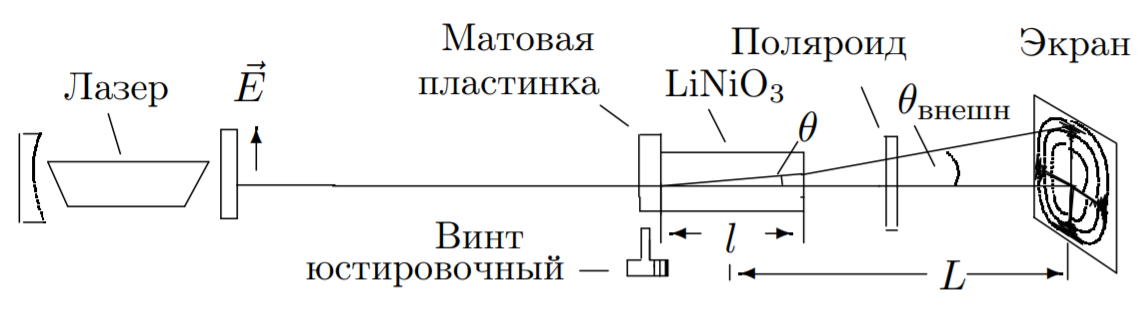
\includegraphics[scale=0.7]{1.png}
		\centering
		\caption{Схема для наблюдения интерфереционной картины.}
	\end{figure}

	Если перед кристаллом, помещённым между поляроидами, расположить линзу или матовую пластинку, то на экране за поляроидом мы увидим тёмные концентрические окружности -- рещультат интерфернции обыкновенной и необыкновенной волн. При повороте выходного поляроида на $90^\circ$ картина меняется с позитива на негатив (на месте светлых пятен тёмные и наоборот). В случаи, когда разрешённое направление анализатора перпендикулярно поляризации лазерного излучения, радиус тёмного кольца с номером $m$ равен
	\begin{equation}
		r_m^2 = \dfrac{\lambda}{l} \dfrac{(n_oL)^2}{n_0 - n_e}m,
	\end{equation}
	где $L$ -- расстояние от центра кристалла до экрана, $l$ -- длина кристалла.\\
	Теперь поместим кристалл в постоянное электрическое поле $E_{\text{эл}}$, направленное вдоль оси $X$, перпендикулярной $Z$. Показатель преломления для луча, распространяющего вдоль $Z$, всегда $n_o$. В плоскости $(X,Y)$ возникают два главных направления под углами $45^\circ$ к $X$ и $Y$ с показателями преломления $n_0 - \Delta n$ и $n_o + \Delta n$ (быстрая и медленная ось), причём $\Delta n = A E_{\text{эл}}$. Для поляризованного вертикально света и анализатора, пропускающего горизонтальную поляризацию, на выходе интенсивность на выходе будет иметь вид
	\begin{equation}
		I_{\text{вых}} = I_0 \sin^2 \left(\dfrac{\pi}{2} \dfrac{U}{U_{\lambda/2}} \right),
	\end{equation}
	где $U_{\lambda/2} = \frac{\lambda}{4A}\frac{d}{l}$ -- \textit{полуволновое напряжение}, $d$ -- поперечный размер кристалла.  При напряжении $U = E_{\text{эл}}d$ равном полуволновому сдвиг фаз между двумя волнами равен $\pi$, а интенсивность света на выходе максимальна. 
	
	 \begin{figure}[h]
		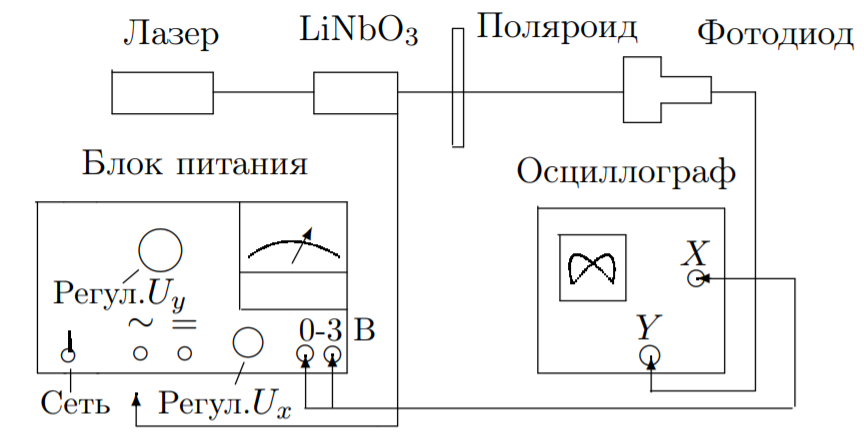
\includegraphics[scale=0.7]{2.png}
		\centering
		\caption{Схема установки}
	\end{figure}
	
	На Рис. 2 представлена схема всей установки (оптическая часть изорбажена на Рис. 1). Свет лазера, проходя через сквозь пластину, рассеивается и падает на двоякопреломляющий кристалл. На экране за поляроидом видна интерференционная картина. Убрав рассеивающую пластину и подавая на кристалл постоянное напряжение, можно величиной напряжения влиять на поляризацию луча, вышедшего из кристалла. Заменив экран фотодиодом и подав на кристалл переменное напряжение, можно исследовать поляризацию с помощью осциллографа.\\
	
	\newpage
	
	\textbf{Ход работы: }\\
	
	\begin{enumerate}
		
	\item Измерим радиусы тёмных колец $r(m)$ и расстояние L от середины кристалла до экрана. Построим график $r^2 = f(m) $. По углу наклона прямой определим двулучепреломление $(n_o - n_e)$ ниобата лития, пользуясь формулой (2). При L = 75,3$\pm 0,1$ см получили следующие радиусы колец:
	
	\begin{longtable}{|c|c|c|c|c|c|c|}
	\hline
	$m$     & 1   & 2   & 3   & 4   & 5   & 6 \\ \hline
	$r_m$, см & 2,4 & 3,4 & 4,3 & 5,1 & 5.7 & 6,3 \\ \hline
	\caption{Радиусы темных колец интерференционной картины. $\sigma_{r_m} = 0,1\text{см}$}
	\end{longtable}

	 \begin{figure}[h]
		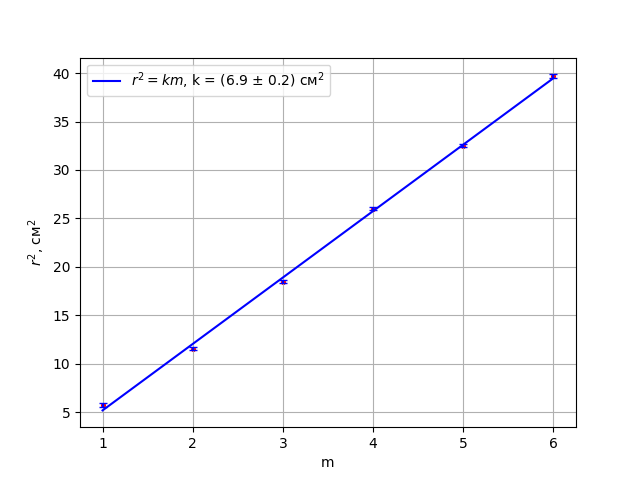
\includegraphics[scale=0.7]{km.png}
		\centering
		\caption{График зависимости $r^2 = f(m)$}
	\end{figure}
	
	$$
	 n_0 - n_e = \dfrac{\lambda}{l} \dfrac{(n_oL)^2}{r_m^2}m = 0,104 \pm 0,003
	$$
	
	\item Получим значения напряжения, при которых интенсивность пятна минимальна и максимальна для двух положений поляроида.
	
	
	\begin{longtable}{|c|c|c|c|}
		\hline
		 & $U_{\lambda/2}$, В & $U_{\lambda}$, В & $U_{\lambda 3/2}$, В \\ \hline
		$\perp$ & 450 & 930 & 1380 \\ \hline
		$\parallel$ & 1035 & 510 & 1500 \\ \hline
		\caption{Значения напряжения для минимумов и максимумов интерференционной картины. $\sigma_U = 15$ В}
	\end{longtable}
	
	
	\begin{figure}[H]
		\centering
		\begin{minipage}[b]{0.4\textwidth}
			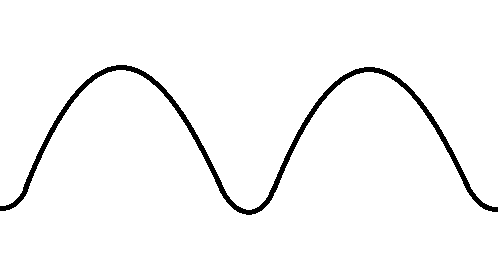
\includegraphics[width=\textwidth]{perp1.png}
			\caption{Фигура Лиссажу для $U_{\lambda}^{\perp}$}
		\end{minipage}
		\hfill
		\begin{minipage}[b]{0.4\textwidth}
			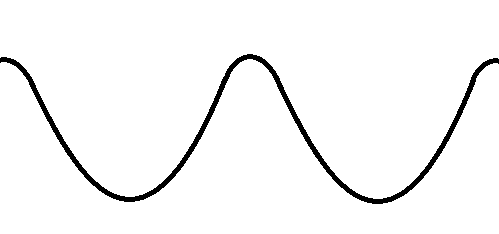
\includegraphics[width=\textwidth]{parall1.png}
			\caption{Фигура Лиссажу для $U_{\lambda}^{\parallel}$}
		\end{minipage}
	\end{figure}
	
	\begin{figure}[H]
		\centering
		\begin{minipage}[b]{0.3\linewidth}
			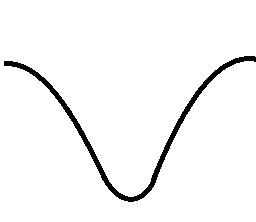
\includegraphics[width=\textwidth]{perp1-2.png}
			\caption{Фигура Лиссажу для $U_{\lambda/2}^{\perp}$}
		\end{minipage}
		\hfill
		\begin{minipage}[b]{0.3\linewidth}
			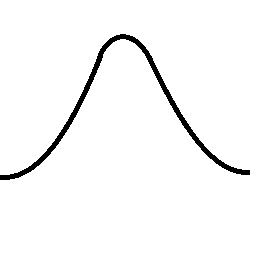
\includegraphics[width=\textwidth]{parall1-2.png}
			\caption{Фигура Лиссажу для $U_{\lambda/2}^{\parallel}$}
		\end{minipage}
	\end{figure}
	
	\begin{figure}[H]
		\centering
		\begin{minipage}[b]{0.45\textwidth}
			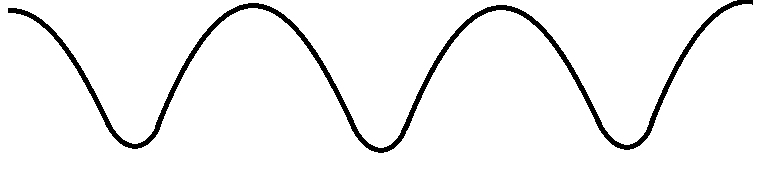
\includegraphics[width=\textwidth]{perp3-2.png}
			\caption{Фигура Лиссажу для $U_{3\lambda/2}^{\perp}$}
		\end{minipage}
		\hfill
		\begin{minipage}[b]{0.45\textwidth}
			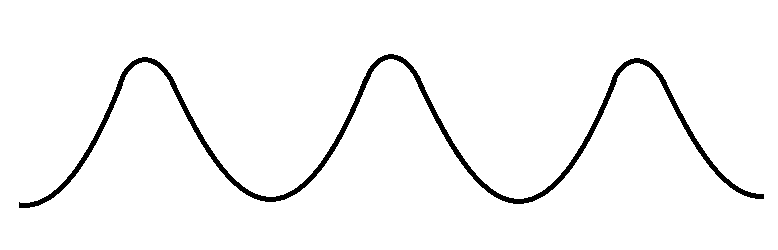
\includegraphics[width=\textwidth]{parall3-2.png}
			\caption{Фигура Лиссажу для $U_{3\lambda/2}^{\parallel}$}
		\end{minipage}
	\end{figure}
	
	\end{enumerate}
	
	\textbf{Обсуждение результатов и выводы: }\\
	
	В ходе данной работы мы исследовали интерференцию рассеянного света,
	прошедшего кристалл, наблюдали изменение характера поляризации света при наложении на кристалл электрического поля.
	
	Определили двулучепреломление $(n_o - n_e) =  0,104 \pm 0,003$ и  полуволновое напряжение  ниобата лития $U_{\lambda/2} = 475 \pm 15$ В. 
	
	
	\end{document}